\documentclass[varwidth=false, border=2pt]{standalone}

\usepackage{tikz}
\usetikzlibrary{arrows,positioning} 
\usetikzlibrary{decorations.markings}
\usetikzlibrary{decorations.pathmorphing}
\usetikzlibrary{fadings}

\begin{document}
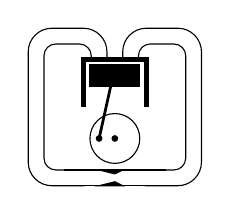
\begin{tikzpicture}


% Pipes
\draw[rounded corners=3mm] (-1.1,-1) rectangle (-0.1,1);
\draw[rounded corners=1.5mm] (-0.9,-0.8) rectangle (-0.3,0.8);
\draw[rounded corners=3mm] (0.1,-1) rectangle (1.1,1);
\draw[rounded corners=1.5mm] (0.3,-0.8) rectangle (0.9,0.8);
\draw[white, fill=white] (-0.6,-1.0) rectangle (0.6,0.6);
\draw (-0.65,-1.0) -- (0.65,-1.0);
\draw (-0.65,-0.8) -- (0.65,-0.8);

% Zylinderkopf
\draw[line width=2pt] (-0.4,0) --(-0.4,0.6) --(0.4,0.6) -- (0.4,0);


% Zylinder
\draw[line width=8pt] (-0.325,0.4) --++(0.65,0);

% Schwungrad
\draw[fill=white] (0,-0.4) circle (9pt);
\draw[fill=black] (0,-0.4) circle (1pt);

% Kurbelgestänge
\draw[line width=1pt] (0,0.5) -- (-0.2,-0.4);
\draw[fill=black] (-0.2,-0.4) circle (1pt);

% Expansionsventil
\draw[fill=black] (-0.2,-0.8) -- (0.1,-0.8)--(0,-0.85) -- cycle;
\draw[fill=black] (-0.2,-1) -- (0.1,-1)--(0,-0.95) -- cycle;



\end{tikzpicture}
\end{document}